\section{Motor}

Nesta secção pretende-se descrever três pontos essenciais desta fase: as
estruturas de dados, algoritmos e processos de \emph{rendering}.


\subsection{Estruturas de Dados}
\label{subsec:sec2}

Como a estrutura do ficheiro XML é uma árvore \emph{n-ária} escolheu-se uma
estrutura que se seguiu a mesma lógica. Assim construiu-se um tipo de dados,
a partir de um \emph{struct} com vários campos para guardar os valores de cada
grupo, onde se encontra um vetor de apontadores para outras estruturas deste
tipo \texttt{Group}, como se pode ver na \emph{Figura~\ref{fig:ssec2:strut}}.
Além do mais, a estrutura base possui um vetor de \emph{strings} para guardar
os nomes de modelos que se encontrarem descritos no ficheiro XML.\ Existe também,
um outro vetor para guardar apontadores de objetos do tipo
\texttt{Transformation}, que representa de forma genérica qualquer transformação
geométrica.

\begin{center} 	
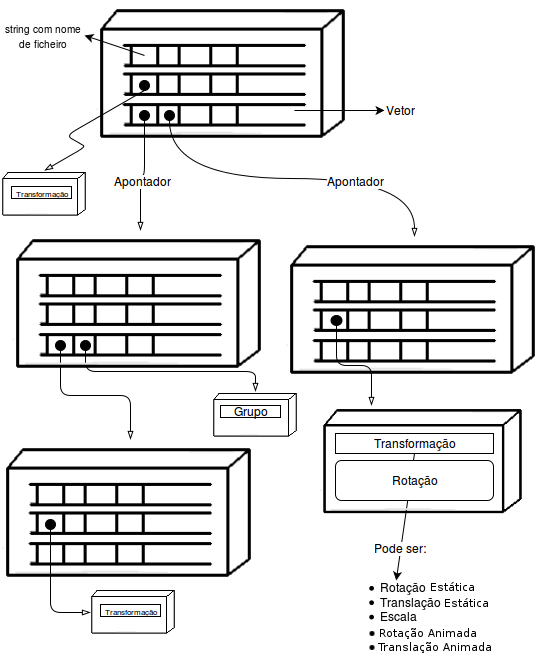
\includegraphics[width=\textwidth,height=\textheight,keepaspectratio]{resources/estrutura.png}
\captionsetup{type=figure, width=0.8\linewidth}
\caption{Árvore \emph{n-ária} para armazenamento de grupos}
\label{fig:ssec2:strut} 
\end{center}

Para a representação genérica de qualquer transformação geométrica, criou-se
uma estrutura de classes, onde a classe \texttt{Transformation} funciona como
superclasse abstrata, com três subclasses: \texttt{Rotation},
\texttt{Translation} e \texttt{Scale}. A superclasse possui um método virtual
para aplicação da transformação (\texttt{applyTrasformation}), que é aplicado no
contexto das suas subclasses quando invado diretamente, ou como parte da
estrutura da hierarquia, à custa do polimorfismo que a linguagem de programação
C++ permite. Esta hierarquia pode ser vista com mais detalhe na
\emph{Figura~\ref{fig:ssec2:class}}. Parte da estrutura de classes é a classe
\texttt{Point3d} que representa um triplo de \texttt{doubles} para as
coordenadas geométricas de um ponto em 3 dimensões. Adicionalmente a classe
implementa alguns métodos para cálculos de pontos e vetores, embora
o significado seja diferente entre estes dois conceitos.

Por último criou-se uma outra estrutura, em que se denominou o tipo
\texttt{Modelos}, que é composta por um apontador para a raiz da árvore
\emph{n-ária} já mencionada, um vetor de \texttt{Triangles}, que
possuirão os dados dos pontos a serem desenhados. A classe \texttt{Triangles}
é composta por três \texttt{Point3d}, representando os três vértices de um
triângulo. O uso daquele vetor é uma medida de eficiência em memória, uma vez
que uma cena pode ser composta por objetos criados com o mesmo conjunto de
pontos, sendo aplicadas transformações para o efeito desejado.

\begin{center} 	
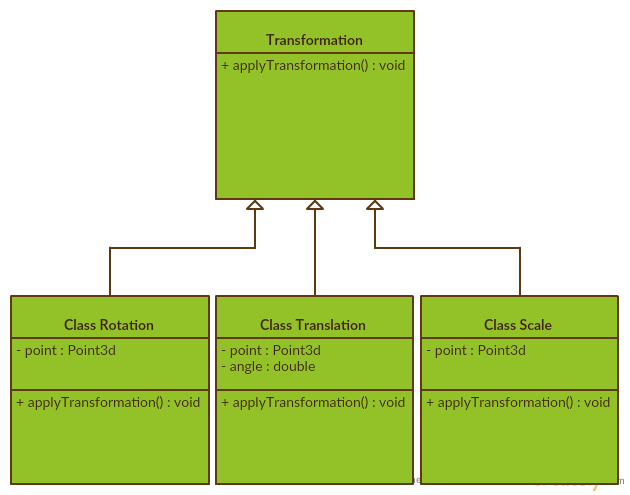
\includegraphics[width=\textwidth,height=\textheight,keepaspectratio]{resources/classes.png}
\captionsetup{type=figure, width=0.8\linewidth}
\caption{Hieraquia de classes de transformações geométricas}
\label{fig:ssec2:class} 
\end{center}
\subsection{Descrição do processo de leitura}

A função principal de leitura é a que está demonstrada no
\emph{Algoritmo~\ref{alg:ssec2:leitura}} e representa parte do processo de
leitura, no entanto decidiu-se remover partes acessórias de inicialização de
estruturas e afins. Esta função serve-se da estrutura de apontadores da árvore
que compõem a estrutura do documento XML para navegar na estrutura
recursivamente. 

Para além do apontador para o estrutura XML, passou-se por
parâmetro um apontador para a estrutura \texttt{Modelos}, que contem um
apontador para a raiz da árvore \emph{n-ária} e uma tabela (ou mapa) com os
valores dos pontos para \emph{rendering} com o nome do ficheiro associado
(chave).Note-se que as estruturas em que se guardam valores dos elementos fazem
todas parte de um \texttt{Group}, tanto como o vetor de
\emph{strings} com o valor dos ficheiro, bem como o vetor de transformações
e outros \texttt{Group} no vetor de grupo, o seu acesso é por uma apontador
para \texttt{Group}, exceto os pares chave/valor guardados numa tabela na
estrutura \texttt{Modelos}, com o acesso feito a estrutura por apontador para
a mesma.  

\begin{algorithm}

\caption{Função Principal Leitura}
\label{alg:ssec2:leitura} 
\footnotesize %% Smaller font size.
\begin{algorithmic}[1]
\Procedure{readXMLFromRootElement}{$XMLElement * elem$, $Modelos * models$,
$Group * grupo$}

\If{$elem = NULL$} 

\Return{}

\EndIf{}

\ForAll{$elem \in SIBLINGS$} 

\If{$elem = TRANSLATION \lor elems = SCALE$} 

\Comment{os atributos $x$, $y$, $z$ são alternativos.Se aparecerem é lhes
atribuído um valor. Caso contrário ficam com o valor $0$}

\If{$elem = TRANSLATION$} 

\State{\texttt{Guardar $x$, $y$, $z$ numa transformação como translação}} 
 
\Else{} 

\State{\texttt{Guardar $x$, $y$, $z$ numa transformação como escala}} 
  
\EndIf{}

\ElsIf{$elem = ROTATION$} 

\Comment{os atributos $axis_{x, y, z}$ e $angle$ são alternativos. Se aparecerem
é lhes atribuído um valor. Caso contrário ficam com o valor $0$}

\State{\texttt{Guardar $axis_{x, y, z}$ e $angle$ numa transformação como
rotação}}

\ElsIf{$elem = MODELS$} 
 
\ForAll{$model \in MODELS$} 

\State{\texttt{Guardar atributo $file$ no vetor de vector<\emph{string}>
apontado por $grupo$}} 

\State{\texttt{Carregar lista de triângulos num $map$ associado a $file$,
apontados por $models$}}

\EndFor{}

\ElsIf{$elem = GROUP$} 

\State{\texttt{Criar novo $* novo\_grupo$}}

\State{\Call{readXMLFromRootElement}{$elem$, $novo\_grupo$}} 
 
\EndIf{}

\EndFor{}

\EndProcedure{}

\end{algorithmic}
\end{algorithm}

Como se pode ver no \emph{Algoritmo~\ref{alg:ssec2:leitura}}, as primeira
instruções referem-se ao caso de paragem da função recursiva que verifica se
o apontador do elemento, representa é um apontador não nulo. Em caso de nulo,
a função retorna para o sítio de onde foi invocada. 
Em seguida itera-se cada elemento que esteja no mesmo nível da árvore do
documento XML.\ podendo o elemento representar uma rotação, uma escala, uma
translação, um modelos ou grupos de modelos, e por fim um grupo.

Com efeito, se o elemento encontrado representar uma escala ou uma
translação obtêm-se os atributos \emph{x}, \emph{y} e \emph{z} e cria-se um
apontador, alocando memória para um instância da classe \texttt{Translation} ou
\texttt{Rotation} com esse valores, conforme a sua existência. Note-se que no
algoritmo, se descreveu de forma breve como se processa cada atributo, ou seja,
cada a existência de cada atributo é verificada, sendo lhe atribuído o valor que
figura na \emph{tag} caso exista, ou \emph{0} caso contrário. 

Por outro lado, se o elemento XML representar uma rotação, cria-se um apontador
alocando memória para um instância da classe \texttt{Rotation}, com os valores
\emph{axisX}, \emph{axisY}, \emph{axisZ} e \emph{angle}. Uma vez mais,
a existência deste atributos é verificada, sendo o valor por defeito \emph{0},
o valor contido na \emph{tag}. 

Há que fazer notar que, um objeto \texttt{Rotation}, \texttt{Translation} ou
\texttt{Scale} são guardados, imediatamente a serem criados, no vetor de
\texttt{Transformation}, que é a superclasse dos tipos anteriores.
O \emph{upcast} é imediato e é uma das caraterísticas da linguagem e de uma
hierarquia de classes. 

Se o elemento representar um conjunto de modelos, é efetuada uma navegação por
apontador para todos os elementos desse conjunto, obtendo o valor do atributo
\emph{file}. Este é guardado no vetor de vetor de \emph{strings} de
\texttt{Group}. De igual modo, através do valor do ficheiro é feita uma leitura
do mesmo, que tem os valores dos pontos dos vértices dos triângulos para
\emph{rendering}. Note-se que cada linha do ficheiro representa um triângulo,
dado que cada linha tem os valores dos vértices separados por ponto e vírgula,
e cada vértice tem as coordenadas \emph{x}, \emph{y} e \emph{z} separadas por
vírgula. Após o \emph{parsing} da linha os valores são inseridos em instâncias
de objetos \texttt{Triangle}, que por sua vez serão adicionados a um vetor.
Aqui é verificada a existência do nome do ficheiro no conjunto de chaves da
tabela, e inserido o par nome do ficheiro/vetor de triângulos no \emph{map} ou
tabela.      

Por último, caso seja encontrado um elemento grupo, podem ocorrer uma de duas
situações: se o grupo está ao mesmo nível do grupo que antecedeu, ou seja é um
elemento \emph{irmão} ou se está dentro de um grupo, isto é, é um \emph{filhos}
do grupo anterior. No entanto, note-se que não existe uma verificação dos dois
caso no algoritmo, sendo efetuada uma chamada recursiva, com um novo elemento
grupo. Para ilustrar o caso, atente-se na
\emph{Figura~\ref{fig:ssec2:recleitura}}. A primeira invocação deste função,
representada pelo algoritmo, é precedida pela inicialização de um
\texttt{Group}, sendo este passado como parâmetro para esta função. Ou seja
é a raiz da árvore de \texttt{Group} e não possui quaisquer valores. O primeiro
elemento que a função encontra é um grupo, como se pode ver na figura, logo tem
que ser inicializado e adicionado à raiz, e apontador deste novo \texttt{Group}
é passado por parâmetro para a chamada recursiva da função. Dentro da chamada
recursiva, vão sendo adicionadas as transformações e modelos e se houver um novo
grupo, o processo repete-se. Algo de salientar é que a raiz, não tem
transformações nem modelos nos respetivos, nunca, e apenas o vetor com os
apontadores para os filhos é que é preenchido. Dado que um elemento com
a \emph{tag} \texttt{scene} pode apenas ter grupos e não transformações, assim
se justifica a raiz não ter transformações. Para o caso da
\emph{Figura~\ref{fig:ssec2:recleitura}}, a raiz terá apenas um \emph{filho},
que será o \emph{pai} de todos os outros grupos.   

À medida que vão sendo encontrados elementos XML nulos, ou seja, que não há mais
nada no mesmo nível, a função ainda entra na chamada recursiva, mas logo
retorna. Para clarificar, o \texttt{Group} para qual foi criada memória, logo
antes desta chamada recursiva tem de existir e é uma folha. Além do mais, como
demonstra a figura, as sucessivas chamadas recursivas vão retornando e voltando
para o sítio onde forma invocadas. Nesta chamadas recursivas, como o apontador
para o \texttt{Group} pai permanece localmente nessa função, vão sendo
adicionados novos os \emph{irmãos}. 

\begin{center}
\includegraphics[scale=0.75,keepaspectratio]{resources/exampleXML.png}
\captionsetup{type=figure, width=0.8\linewidth}
\caption{Diagrama representativo da recursividade do processo de leitura}
\label{fig:ssec2:recleitura} 
\end{center}


\newpage
\subsection{Descrição do ciclo de \emph{rendering}}



Para fazer o \emph{rendering} da estrutura de dados em memória, implementou-se
uma função de travessia da árvore, colocada na função \texttt{renderScene}, após
a função \texttt{glLoadIndentity} e \texttt{gluLookAt}, nesta sequência.
O \emph{Algoritmo~\ref{alg:ssec2:traverse}} representa a função que efetua esta
travessia.

Com efeito, a primeira instrução é a \texttt{glPushMatrix}, uma vez que se
pretende colocar uma matriz para aplicação das transformações no topo da
\emph{stack} de matrizes do \emph{OpenGL}. Em seguida, para cada transformação
contida num \texttt{Group}, é invocada a função \texttt{applyTrasformation}, já
mencionada na \emph{Secção~\ref{subsec:sec2}}, que aplica as transformações
conforme o contexto, como já foi explicado.

Em seguida, é invocada a função \texttt{drawElement}, descrita no
\emph{Algoritmo~\ref{alg:ssec2:rendering}}. Esta função especifica a primitiva
para que será criada com os vértices em memória, neste caso com um triplo de
vértices. Os vértices estão contidos, em objetos do tipo \texttt{Triangle} que
por sua vez, contêm objetos do tipo \texttt{Point3d} com as coordenadas de cada
vértice. Para obter estes vértices e criar a primitiva com \texttt{glVertex3f},
é necessário obtêm todas as \emph{strings} com o nome dos ficheiros no vetor de \emph{string} de cada \texttt{Group}. Como cada nome, procura-se pelo
nome de ficheiro na tabela a partir do apontador para \texttt{Modelos}. Se
a entrada existir, obtêm-se todos valores de \texttt{Triangle}, respetivos
vértices e coordenadas.

No seguimento desta instrução existe um ciclo para aceder a elementos do vetor
de apontadores pelo índice para \texttt{Group}. Cada elemento (apontador para
\texttt{Group}) em determinada posição do \emph{array} é passado por argumento
para a chamada recursiva da função. Quando o chamada recursiva retorna, o índice
é incrementado e o processo repete-se.\ A função termina quando não houver mais
elementos no vetor.  Ou seja, o índice é incrementando à medida que
a chamadas recursivas entram na memória automática (\emph{stack}) e retornam,
saindo da \emph{stack}. 

Por último, note-se que a \texttt{glPopMatrix} é executada logo após o retorno
da chamada recursiva. Uma vez que as transformações sejam herdadas é necessário
colocar matrizes na \emph{stack} de matrizes do \emph{OpenGL}, conforme se vai
descendo na árvore. Quando a função faz o \emph{pop} à \emph{stack} de matrizes,
faz-lo na mesma chamada recursiva da função.

\newpage

\begin{algorithm}
\caption{Função de travessia da árvore de \texttt{Group}}
\label{alg:ssec2:traverse} 
\footnotesize %% Smaller font size.
\begin{algorithmic}[1]

\Procedure{traverseTree}{$Modelos * models$, $Group *grupo$}

\State{\Call{glPushMatrix}{$~$}} 

\ForAll{$transformation \in grupo \to TRANSFORMATIONS$} 
 
\State{$transformation\to \Call{applyTransformation}{ }$} 
 
\EndFor{}

\State{\Call{drawElement}{$models$, $grupo$}} 

\State{$i \gets 0$} 

\While{$i < $ tamanho do \emph{array} $grupo \to FILHOS$}

\State{\Call{traverseTree}{$models$, $grupo\to FILHOS_{i}$}} 

\State{\Call{glPopMatrix}{$~$}} 

\State{$i \gets i = i + 1$}

\EndWhile{}

\EndProcedure{}

\end{algorithmic}
\end{algorithm}
%%%%%%%%%%%%%%%%%%%%%%%%%%%%%%%%%%%%%%%%%%%%%%%%%%%%%%%%%%

\begin{algorithm}

\caption{Função de \emph{rendering} dos pontos}
\label{alg:ssec2:rendering} 
\footnotesize %% Smaller font size.
\begin{algorithmic}[1]

\Procedure{drawElement}{$Modelos * models$, $Group *grupo$}

\State{\Call{glBegin}{GL\_TRIANGLES}} 



\ForAll{\emph{String} $\in$ vetor de \emph{strings} pontado
por $grupo$} 

\State{Procurar $entry$ com a \emph{string} (nome do ficheiro), no $map$
apontado por $models$} 

\If{$entry$ existe}

\ForAll{Triângulo $ABC$ $\in$ valores (\texttt{vetor} de triângulos) associado
à chave} 
 
\State{Obter vértices do triângulo $ABC$}

\State{\Call{glVertex3f}{$xA$, $yA$, $zA$}}

\State{\Call{glVertex3f}{$xB$, $yB$, $zB$}}

\State{\Call{glVertex3f}{$xC$, $yC$,$zC$}}
 
\EndFor{}

\EndIf{}
 
\EndFor{}

\State{\Call{glEnd}{$~$}} 

\EndProcedure{}
\end{algorithmic}
\end{algorithm}

